\documentclass[fleqn, a4paper, 12pt, twoside]{article}

\newcounter{recitationcount} %creates a new counter for recitation numbers (must be executed before exsheets is loaded)
\newcommand\recitation{\refstepcounter{recitationcount}}

\usepackage[counter-within = recitationcount]{exsheets}
\usepackage{amsmath, amssymb, amsthm} %standard AMS packages
\usepackage{marginnote} %marginnotes
\usepackage{gensymb} %miscellaneous symbols
\usepackage{commath} %differential symbols
\usepackage{xcolor} %colours
\usepackage{cancel} %cancelling terms
\usepackage{siunitx} %formatting units
\usepackage{tikz, pgfplots} %diagrams
	\usetikzlibrary{calc, hobby, patterns, intersections}
\usepackage{graphicx} %inserting graphics
\usepackage{hyperref} %hyperlinks
\usepackage{datetime} %date and time
\usepackage{ulem} %underline for \emph{}
\usepackage{xfrac, lmodern} %inline fractions
\usepackage{enumerate} %numbered lists
\usepackage{float} %inserting floats
\usepackage{circuitikz} %circuit diagrams

\newcommand\numberthis{\addtocounter{equation}{1}\tag{\theequation}} %adds numbers to specific equations in non-numbered list of equations

\newcommand{\AxisRotator}[1][rotate=0]{
	\tikz [x=0.25cm,y=0.60cm,line width=.2ex,-stealth,#1] \draw (0,0) arc (-150:150:1 and 1);%
} %rotation symbols on axes

\theoremstyle{definition}
\newtheorem{example}{Example}
\newtheorem{definition}{Definition}

\theoremstyle{theorem}
\newtheorem{theorem}{Theorem}

\newcommand{\curl}{\mathrm{curl\,}}

\makeatletter
\@addtoreset{section}{part} %resets section numbers in new part
\makeatother

\newcommand\blfootnote[1]{%
	\begingroup
	\renewcommand\thefootnote{}\footnote{#1}%
	\addtocounter{footnote}{-1}%
	\endgroup
}

\RenewQuSolPair{question}[name=Recitation \therecitationcount\ -- Exercise]{solution}[name=Recitation \therecitationcount\ -- Solution]

\SetupExSheets{solution/print = true, totoc = true} %prints all solutions by default

%opening
\title{Differential and Integral Calculus : Recitations}
\author{Aakash Jog}
\date{2014-15}

\begin{document}

\maketitle
%\setlength{\mathindent}{0pt}

\blfootnote
{	
	\begin{figure}[H]
		
\includegraphics[height = 12pt]{cc.eps}
		\includegraphics[height = 12pt]{by.eps}
		\includegraphics[height = 12pt]{nc.eps}
		
\includegraphics[height = 12pt]{sa.eps}
	\end{figure}
	This work is licensed under the Creative Commons Attribution-NonCommercial-ShareAlike 4.0 International License. To view a copy of this license, visit \url{http://creativecommons.org/licenses/by-nc-sa/4.0/}.
} %CC-BY-NC-SA licencse

\tableofcontents

\newpage
\section{Instructor Information}

\textbf{Michael Bromberg}\\
~\\
E-mail: \href{mailto:micbromberg@gmail.com}{micbromberg@gmail.com}\\

\newpage

\part{Sequences and Series}

\section{Sequences}

\recitation

\begin{question}
	Prove:
	\begin{equation*}
		\lim\limits_{n \to \infty} \dfrac{2n^2 + n + 1}{n^2 + 3} = 2
	\end{equation*}
\end{question}

\begin{solution}[print]
	Let
	\begin{equation*}
		\varepsilon > 0
	\end{equation*}

	\begin{align*}
		\left| \dfrac{2n^2 + n + 1}{n^2 + 3} - 2 \right| &= \left| \dfrac{2n^2 + n + 1 - 2n^2 - 6}{n^2 + 3} \right|\\
		&= \left| \dfrac{n - 5}{n^2 + 3} \right| \\
		&\leq \left| \dfrac{n - 5}{n^2} \right|\\
		&\leq \dfrac{1}{n}\\
		&< \varepsilon
	\end{align*}
	Therefore, let $N = \left[ \dfrac{1}{\varepsilon} \right] + 1$.
	Hence, for this $N$, $|a_n - L| < \varepsilon$.\\
	Therefore, $\lim\limits_{n \to \infty} \dfrac{2n^2 + n + 1}{n^2 + 3} = 2$.
	\qed
\end{solution}

\begin{question}
	Prove
	\begin{equation*}
		\lim\limits_{n \to \infty} \dfrac{n^3 + \sin n + n}{2n^4} = 0
	\end{equation*}
\end{question}

\begin{solution}[print]
	Let $\varepsilon > 0$
	\begin{align*}
		\left| \dfrac{n^3 + \sin n + n}{2n^4} \right| &\leq \left| \dfrac{n^3 + 1 + n}{2n ^4} \right|\\
		&\leq \left| \dfrac{3n^3}{2n^4} \right| = \dfrac{3}{2} \cdot \dfrac{1}{n} < \varepsilon
	\end{align*}
	Therefore, let $N = \left[ \dfrac{3}{2 \varepsilon} \right] + 1$.
	Hence, for this $N$, $|a_n - L| < \varepsilon$.\\
	Therefore, $\lim\limits_{n \to \infty} \dfrac{n^3 + \sin n + n}{2n^4} = 0$
	\qed
\end{solution}

\begin{question}
	Calculate $\sqrt[3]{n^3 + 3n} - n$.
\end{question}

\begin{solution}[print]
	\begin{align*}
		a^n - b^n = (a - b) \cdot (a^{n - 1} + a^{n - 2} b + \dots + a b^{n - 2} + b^{n - 1})
	\end{align*}
	Therefore, let
	\begin{align*}
		a &= \sqrt[3]{n^3 + 3n}\\
		b &= \sqrt[3]{n^3}
	\end{align*}

	\begin{align*}
		a - b &= \dfrac{a^3 - b^3}{a^2 + a b + b^2}\\
		\therefore \sqrt[3]{n^3 + 3n} - n &= \dfrac{n^3 + 3n - n^3}{(n^3 + 3n)^{\sfrac{2}{3}} + (n^3 + 3n)^{\sfrac{1}{3}} n + n^2}\\
		&= \dfrac{3}{\left( \dfrac{n^3 + 3n}{n^{\sfrac{3}{2}}} \right)^{\sfrac{2}{3}} + \left( \dfrac{n^3 + 3n}{n^3} \right)^{\sfrac{1}{3} n} + n}
	\end{align*}
	Therefore, the limit is 0.
\end{solution}

\begin{question}
	Prove
	\begin{equation*}
		\lim\limits_{n \to \infty} \dfrac{n!}{n^n} = 0
	\end{equation*}
\end{question}

\begin{solution}[print]
	\begin{equation*}
		0 \leq \dfrac{n!}{n^n} = \dfrac{1}{n} \dfrac{2}{n} \dots \dfrac{n}{n} \leq \dfrac{1}{n}\\
	\end{equation*}
	Therefore, by the Sandwich Theorem, $\lim\limits_{n \to \infty} \dfrac{n!}{n^n} = 0$.
\end{solution}

\begin{question}
	Let $a_1 = 3$, $a_{n + 1} = 1 + \sqrt{6 + a_n}$. Prove that $a_n$ converges and find its limit.
\end{question}

\begin{solution}[print]
	If possible, let $\lim\limits_{n \to \infty} a_n = l$.
	\begin{align*}
		a_{n + 1} &= 1 + \sqrt{6 + a_n}\\
		\intertext{Taking the limit on both sides,}
		l &= 1 + \sqrt{6 + l}\\
		\therefore l - 1 &= \sqrt{6 + l}\\
		\therefore l &= \dfrac{3 \pm \sqrt{29}}{2}
	\end{align*}
	As $a_n \geq 0$, $l = \dfrac{3 + \sqrt{29}}{2}$.
	~\\
	\begin{align*}
		a_2 &= 1 + \sqrt{6 + a_1}\\
		&= 1 + \sqrt{6 + 3}\\
		&= 4\\
		\therefore a_2 &> a_1
	\end{align*}
	If possible, let $a_n \geq a_{n - 1}$.\\
	Therefore,
	\begin{align*}
		a_{n + 1} &= 1 + \sqrt{6 + a_n}\\
		&\geq 1 + \sqrt{6 + a_{n + 1}} = a_n
	\end{align*}
	Therefore by induction, $\{a_n\}$ is monotonically increasing.
	~\\
	\begin{align*}
		a_1 &= 3\\
		\therefore a_1 \leq 5
	\end{align*}
	If possible, let $a_n \leq 5$.\\
	Therefore,
	\begin{equation*}
		a_{n + 1} = 1 + \sqrt{6 + a_n} \leq q + \sqrt{11} \leq 5
	\end{equation*}
	Therefore by induction, $\{a_n\}$ is bounded from above by 5.
\end{solution}

\recitation

\subsection{Limit of a Function by Heine}

\begin{definition}
	\begin{equation*}
		\lim\limits_{x \to x_0} f(x) = l
	\end{equation*}
	if for every sequence $x_n$, such that $\lim\limits_{n \to \infty} x_n = x_0$, \begin{equation*}
		\lim\limits_{n \to \infty} f(x_n) = l
	\end{equation*}
\end{definition}

\begin{theorem}
	If $f$ is continuous at $x_0$ and $x_n \to x_0$, then 
	\begin{equation*}
		\lim\limits_{n \to \infty} f(x_n) = f\left( \lim\limits_{n \to \infty} x_n \right) = f_{x_0}
	\end{equation*}
\end{theorem}

\begin{question}
	Calculate $\lim\limits_{n \to \infty} \sqrt[n]{n}$.
\end{question}

\begin{solution}
	Let
	\begin{equation*}
		f(x) = x^{\sfrac{1}{x}}
	\end{equation*}
	Therefore,
	\begin{align*}
		\lim\limits_{x \to \infty} x^{\sfrac{1}{x}} &= \lim\limits_{x \to \infty} e^{\cancelto{0}{\dfrac{\ln x}{x}}}\\
		&= 1
	\end{align*}
\end{solution}

\subsection{Sub-sequences}

\begin{question}
	Find all partial limits and $\overline{\lim}$ and $\underline{\lim}$ of
	\begin{equation*}
		a_n = \left( \cos \dfrac{\pi n}{4} \right)^n
	\end{equation*}
\end{question}

\begin{solution}
	Let $k, z \in \mathbb{Z}$
	\begin{align*}
		\cos \dfrac{\pi n}{4} &= \cos \dfrac{\pi (n + k)}{4}\\
		\therefore \dfrac{\pi n}{4} &= \dfrac{\pi (n + k)}{4} + 2 \pi z\\
		\therefore \pi n &= \pi (n + k) + 8 \pi z\\
		\therefore k &= 8 z
	\end{align*}
	Therefore,
	\begin{align*}
		a_{8k} &= \left( \cos \dfrac{\pi \cdot 8k}{4} \right)^{8k}\\
		&= \left( \cos (2 \pi k) \right)^{8k}\\
		&= 1\\
		a_{8k + 1} &= \left( \cos \dfrac{\pi \cdot (8k + 1)}{4} \right)^{8k + 1}\\
		&= \left( \cos \dfrac{\pi}{4} \right)^{8k + 1}\\
		&= \left( \dfrac{\sqrt{2}}{2} \right)^{8k + 1}\\
		a_{8k + 2} &= \left( \cos \dfrac{\pi \cdot (8k + 2)}{4} \right)^{8k + 2}\\
		&= \left( \cos \dfrac{\pi}{2} \right)^{8k + 2}
	\end{align*}
	Therefore,
	\begin{align*}
		\lim\limits_{k \to \infty} a_{8k} &= 1\\
		\lim\limits_{k \to \infty} a_{8k + 1} &= \lim\limits_{k \to \infty} \left( \dfrac{\sqrt{2}}{2} \right)^{8k + 1}\\
		&= 0
	\end{align*}
	Similarly,
	\begin{align*}
		\lim\limits_{k \to \infty} a_{8k + 2} &= 0\\
		\lim\limits_{k \to \infty} a_{8k + 3} &= 0\\
		\lim\limits_{k \to \infty} a_{8k + 4} &= \lim\limits_{k \to \infty} (-1)^{8k + 4}\\
		&= 1\\
		\lim\limits_{k \to \infty} a_{8k + 5} &= 0\\
		\lim\limits_{k \to \infty} a_{8k + 6} &= 0\\
		\lim\limits_{k \to \infty} a_{8k + 7} &= 0
	\end{align*}
	Therefore, $\{a_n\}$ has two partial limits, $0$ and $1$.
	\begin{align*}
		\overline{\lim} a_n &= 1\\
		\underline{\lim} a_n &= 0
	\end{align*}
\end{solution}

\section{Series}

\begin{definition}[Convergence of a series]
	Let $\{a_n\}$ be a sequence. Let $S_n$ be a sequence of partial sums of $a_n$, s.t.
	\begin{equation*}
		S_n = \sum_{k = 1}^{n} a_k
	\end{equation*}
	The series $\sum_{k = 1}^{\infty} a_k$ is said to converge to $l$ if
	\begin{equation*}
		\lim\limits_{n \to \infty} S_n = l
	\end{equation*}
	that is,
	\begin{equation*}
		\sum_{k = 1}^{\infty} a_k = \lim\limits_{n \to \infty} \sum_{k = 1}^{n} a_k = \lim\limits_{n \to \infty} S_n
	\end{equation*}
\end{definition}

\begin{question}
	Does $\displaystyle \sum_{k = 0}^{\infty} q^k$ where $-1 < q < 1$ converge?
\end{question}

\begin{solution}
	\begin{align*}
		\sum_{k = 0}^{\infty} q^k &= \lim\limits_{n \to \infty} \sum_{k = 0}^{n} q^k\\
		&= \lim\limits_{n \to \infty} \dfrac{1 - q^{n + 1}}{1 - q}\\
		&= \dfrac{1}{1 - q}
	\end{align*}
	Therefore, the series converges.
\end{solution}

\begin{question}
	Does $\displaystyle \sum_{k = 1}^{\infty} \dfrac{1}{k(k + 1)}$ converge?
\end{question}

\begin{solution}
	\begin{align*}
		\sum_{k = 1}^{\infty} \dfrac{1}{k(k + 1)} &= \sum_{k = 1}^{\infty} \left( \dfrac{1}{k} - \dfrac{1}{k + 1} \right)\\
		&= \lim\limits_{n \to \infty} \sum_{k = 1}^{n} \left( \dfrac{1}{k} - \dfrac{1}{k + 1} \right)\\
		&= \lim\limits_{n \to \infty} \left( 1 - \dfrac{1}{n + 1} \right)\\
		&= 1
	\end{align*}
\end{solution}

\begin{question}
	Does $\displaystyle \sum_{k = 1}^{\infty} \left( 1 + \dfrac{1}{k} \right)^k$ converge?
\end{question}

\begin{solution}
	\begin{align*}
		\lim\limits_{k \to \infty} \left( 1 + \dfrac{1}{k} \right)^k &= e\\
		\therefore \lim\limits_{k \to \infty} \left( 1 + \dfrac{1}{k} \right)^k &\neq 0
	\end{align*}
	Therefore, the necessary condition is nt satisfied.
	Hence, the series does not converge.
\end{solution}

\subsection{Comparison Tests for Positive Series}

\begin{theorem}[First Comparison Test]
	If $a_n \ge 0$, $b_n \ge 0$, and $a_n \le b_n$, then
	\begin{enumerate}
		\item If $\sum b_n$ converges, then $\sum a_n$ converges.
		\item If $\sum a_n$ diverges, then $\sum b_n$ diverges.
	\end{enumerate}
	\label{FIrst Comparison Test}
\end{theorem}

\begin{theorem}[Second Comparison Test]
	If $a_n \ge 0$, $b_n \ge 0$ and
	\begin{equation*}
		\lim\limits_{n \to \infty} \dfrac{a_n}{b_n} = l
	\end{equation*}
	where $0 < l < \infty$, then $\sum a_n$ and $\sum b_n$ converge or diverge simultaneously.
	\label{Second Comparison Test}
\end{theorem}

\end{document}
